\begin{figure}[t]
\centering
\resizebox{\linewidth}{!}{%
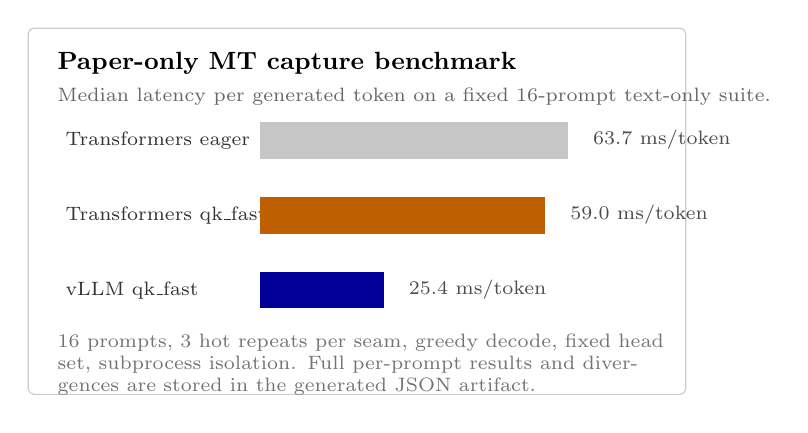
\begin{tikzpicture}[x=1cm,y=1cm, every node/.style={font=\scriptsize}]
\draw[rounded corners=2pt, fill=white, draw=black!20] (0,-0.2) rectangle (8.35,4.45);
\node[anchor=west, font=\bfseries\small] at (0.25,4.00) {Paper-only MT capture benchmark};
\node[anchor=west, text=black!60] at (0.25,3.58) {Median latency per generated token on a fixed 16-prompt text-only suite.};
\node[anchor=west, text=black!80] at (0.35,3.02) {Transformers eager};
\filldraw[fill=gray!45, draw=gray!45] (2.95,2.80) rectangle (6.85,3.25);
\node[anchor=west, text=black!70] at (7.05,3.03) {63.7 ms/token};
\node[anchor=west, text=black!80] at (0.35,2.07) {Transformers qk\_fast};
\filldraw[fill=orange!75!black, draw=orange!75!black] (2.95,1.85) rectangle (6.56,2.30);
\node[anchor=west, text=black!70] at (6.76,2.08) {59.0 ms/token};
\node[anchor=west, text=black!80] at (0.35,1.12) {vLLM qk\_fast};
\filldraw[fill=blue!60!black, draw=blue!60!black] (2.95,0.90) rectangle (4.51,1.35);
\node[anchor=west, text=black!70] at (4.71,1.13) {25.4 ms/token};
\node[anchor=west, text=black!55, align=left, text width=7.7cm] at (0.25,0.18) {16 prompts, 3 hot repeats per seam, greedy decode, fixed head set, subprocess isolation. Full per-prompt results and divergences are stored in the generated JSON artifact.};
\end{tikzpicture}
}
\caption{\textbf{Inference-time comparison of MT capture seams.} We compare a minimal Transformers eager reference, a Transformers qk-fast reference that reconstructs source rows from captured layer inputs, and the engine-native vLLM qk-fast path used by the shipped backend. The main plot reports the median latency per generated token on a fixed 16-prompt benchmark suite, with one unmeasured warmup pass and repeated hot runs per seam.}
\label{fig:mt-capture-speed}
\end{figure}
